\newcommand{\whiteball}{\includegraphics[page=20,scale=0.4]{picsc}}
\newcommand{\blackball}{\includegraphics[page=19,scale=0.4]{picsc}}
\newcommand{\blueball}{\includegraphics[page=21,scale=0.4]{picsc}}
\newcommand{\redball}{\includegraphics[page=22,scale=0.4]{picsc}}



This chapter is about automata which input words and output rational numbers. The original definition comes from Schützenberger~\cite{Schutzenberger:1961cf}. 
We show that these automata can be minimised  (even in  polynomial time) and  can be  tested for equivalence (again, in polynomial time),  but the following version of the emptiness problem is undecidable: 
\begin{center}
	is the output $0$ for at least one input?
\end{center}
 Note that the dual problem, 
 \begin{center}
 	is the output $0$ for all inputs?
 \end{center}
  is a special case of the equivalence problem, and is therefore decidable in polynomial time.  We use the field of rational numbers, but most results would work for other fields. The automata  can be viewed in two ways: as a nondeterministic device with states from a finite set (we call these weighted automata) and as a deterministic device with states from a vector space (we call these vector space automata). Both views are useful, so we present both of them. 

\paragraph*{Weighted automata.} In the nondeterministic view, the automaton has a state space which is a finite set, and many possible runs. Each run has an associated weight, and the weight of an input word is the sum of weights of all the runs.



\begin{definition}[Weighted automaton]\label{def:weighted-automaton}
A \emph{weighted automaton} consists of:
\begin{enumerate}
	\item a finite set $\Sigma$, called the \emph{input alphabet};
	\item a finite set $P$ of \emph{states};
	\item for each state, an \emph{initial weight} and \emph{final weight}, which are rational numbers;
	\item a \emph{transition function} from $P \times \Sigma \times P$ to rational numbers.
\end{enumerate}
Define the \emph{weight} of  a run of the automaton to be the product of: the initial weight of the first state, the  weights of all transitions used, and the final weight of the last state, as in the following picture:
\mypicc{9}
 Define the \emph{weight} of a word to be the sum of the weights of all runs.  The function \emph{recognised} by the automaton is the function that maps a word to its weight.
\end{definition}

The above definition makes sense for an arbitrary semiring, i.e.~a set equipped with product and sum operations, such that sum is commutative and there is an appropriate distributivity law. If we take the semiring 
\begin{align*}
(\underbrace{\set{0,1,2,\ldots,\infty}}_{\text{universe of the semiring}}, \underbrace{\min}_{\text{sum of the semiring}}, \ \underbrace{+}_{\text{product of the semiring}})	
\end{align*}
then we recover distance automata as discussed in Chapter~\ref{sec:distance-automata}. For this chapter, however, it will be important that we use the rational numbers, or more generally a  field, so that we can use linear algebra.


\begin{example}
Consider the following weighted automaton with three states.
\mypicc{7}
 The weight of a run that stays in $\whiteball$  is  $1$, and the weight of a run that goes from $\whiteball$ to $\blackball$  is $2^n$, where $n$ is the number of times the run loops around $\blackball$. Other runs have cost zero. If the input word has length $n$, then the weight of the word is
\begin{align*}
	\underbrace{2^{n-1} + 2^{n-1} + \cdots +2^1}_{\text{runs from $\whiteball$ to $\blackball$}} + \underbrace{1}_{\text{loop in $\whiteball$}} = 2^n
\end{align*}
To recognise the same function $a^n \mapsto 2^n$ we could also use this automaton
\mypicc{10}
As we will see later in this chapter, weighted automata can be minimised. The second automaton is in fact the minimal automaton -- how could it be smaller? -- and there exists an automaton homomorphism  (see later in the chapter for the definition) from  the first automaton to the second one, namely the function
\begin{align*}
  x \cdot \whiteball + y \cdot \blackball \qquad \mapsto \qquad (x+y) \cdot \blueball.
\end{align*}



\end{example}
\begin{example}[Running example] \label{ex:run-wei-one} We describe two weighted automata which will be used as the running example in this chapter.
We can view a nondeterministic automaton  as a special case of a weighted automaton, by assuming that every arrow (including dangling arrows that indicate initial and final states) has weight 1. In this   view,  the  semantics of weighted automata will map an input word  to  the number of accepting runs. 
	Consider the following two nondeterministic automata over input alphabet $\set a$
	\mypicc{11}
	 which both recognise the language ``nonempty words''. Both automata are unambiguous, i.e.~on each accepted word they have exactly one run. Therefore, if we treat the automata  as weighted automata, then the recognised  function will  be the characteristic function of the set of nonempty words. Note that the semantics of weighted automata is finer, i.e.~leads to more non-equivalent automata, than the standard nondeterministic semantics. For example, the automaton
	 \mypicc{24}
	 also recognises -- as a nondeterministic automaton -- the set of nonempty words, but it has $n$ runs on inputs of length $n$, and therefore it is not equivalent to the unambiguous  automata when seen as a weighted automaton.  We will return to the unambiguous  automata later in the chapter, and show that they are isomorphic as weighted automata.
\end{example}

\paragraph*{Vector space automata.} We now present a deterministic view on weighted automata. In this view, the automaton has a  state space that is a vector space, and each letter deterministically updates the state using a linear function. This definition is almost the same as  the original definition of Schützenberger~\cite[Definition 1]{Schutzenberger:1961cf}, except that the original definition also allowed control states from a finite set. We do not use control states, because they do  not contribute to expressive power of the model (although they make constructions easier), see the proof of Lemma~\ref{lem:weighted-closure}.




\begin{definition}[Vector space automaton]\label{def:vector-space-automaton} A  \emph{vector space automaton\footnote{This definition is designed so that it can be generalised to categories other than the category of vector spaces, see e.g.~\cite{Colcombet:2017is}}} consists of:
\begin{enumerate}
	\item an input alphabet, which is a finite set $\Sigma$;
	\item a set $Q$ of states, which is a vector space of finite dimension over $\field$;
	\item an initial state $q_0 \in Q$;
	\item for each letter $a \in \Sigma$, a linear map from $Q$ to itself, denoted by  $q \mapsto qa$;
	\item a linear map from $Q$ to the rational numbers, called the \emph{output function}.
\end{enumerate}
%A vector space automaton is called \emph{finite} if the input alphabet is finite and the vector space has finite dimension\footnote{One could consider a more general definition, where the input alphabet is also a vector space, and the transition function is a bi-linear map $Q \times \Sigma \to Q$. The case of finite input alphabets would be recovered by viewing an input letter as one of the base vectors in the vector space $\field^\Sigma$ of finite dimension.}.
The automaton begins in the initial state, and when reading a letter $a \in \Sigma$, it updates its state using the transition function from item 4. After reading all the letters of the input word, the output function is applied to the last state, yielding the output of the automaton.
\end{definition}

The state space of a vector space automaton is  isomorphic to $\field^n$ for some $n \in \Nat$, since these are the vector spaces of finite dimension. Therefore, when representing a vector space automaton for the use of algorithms, we simply indicate the dimension $n$, and use matrices to represent the transitions from item 4 and the output function from item 5. 


\begin{example}\label{ex:weighted-length} Without increasing the expressive power of the model, we could allow affine functions in the transitions of a vector space automaton.  The construction is illustrated on the following example.

	Consider the length function over a one letter alphabet $\set a$. The most natural approach to recognise this function  would be to have the one dimensional vector space $\field$ as the state space and use the affine function $q \mapsto q+1$ as the transition function. However, Definition~\ref{def:vector-space-automaton} requires linear transition functions, so we use a workaround.
	The state space is $\field^2$ and the initial state is $(1,0)$. When reading a letter $a$, the automaton applies the function
	\begin{align*}
  (x,y) \mapsto (x,x+y)
\end{align*}
and the output function is $(x,y) \mapsto y$. 
As an alternative to the above vector space automaton, we can use the following weighted automaton 
\mypicc{12}
If we ignore the weights, the above picture shows a nondeterministic automaton, which has exactly $n$ accepting runs on a word of the form $a^n$, and thus using the weighted semantics, we get the length function. (This is the weighted automaton at the end of Example~\ref{ex:run-wei-one}.)
\end{example}


\paragraph*{Equivalence of the models.} A closer inspection of the vector space automaton and the weighted automaton used in Example~\ref{ex:weighted-length} shows that these are actually the same automaton, only drawn using different pictures. This sameness is formalised in the following lemma.
\begin{lemma}\label{lem:}
	Weighted automata and vector space automata recognise the same functions.
\end{lemma}
\begin{proof} 
Actually, the proof shows something more, namely that the two definitions of automata are just different syntaxes for the same object. 
To transform between syntaxes, we use the  transformation
\begin{align*}
  \Aa \in \text{weighted automata} \qquad \mapsto \qquad \mathsf{vec}\Aa \in \text{vector space automata},
\end{align*}
described below, 
which preserves the recognised function. The transformation  is easily seen to be reversible, thus proving the lemma. 

The vector space automaton $\mathsf{vec}\Aa$ is defined as follows.
\begin{itemize}
	\item The state space of $\mathsf{vec}\Aa$ is  $\field^P$, where $P$ is the states of $\Aa$.
	\item The initial state of $\mathsf{vec}\Aa$  assigns to each state its initial weight.
	\item The output function of $\mathsf{vec}\Aa$ multiplies each coordinate by its final weight.
	\item For each input letter $a \in \Sigma$,  the state update $q \mapsto qa$ of  $\mathsf{vec}\Aa$   maps a vector $q$ to a vector which stores the following number on coordinate $p \in P$:
  \begin{align*}
 \sum_{r \in P} (\text{coordinate $r$ of $q$}) \cdot (\text{weight of transition $r \stackrel a \to p$ in $\Aa$}).
\end{align*}
An alternative view is that the linear map above is described by the matrix which is obtained by looking at the weights of transitions that read letter $a$ in the automaton $\Aa$.

\end{itemize}
 \end{proof}

\begin{example}[Running example]
Recall the  two weighted automata:
\mypicc{11}
 We now show the corresponding vector space automata. The state spaces of the automata are  2-dimensional vector spaces with bases $\set{\whiteball, \blackball}$ and $\set{\blueball, \redball}$, respectively.
The initial vectors are $\whiteball$ and $\blueball$, respectively, while the transition functions are
\begin{align*}
  (x \cdot \whiteball + y \cdot \blackball) \cdot a = (x+y) \cdot \blackball \qquad  (x \cdot \blueball + y \cdot \redball)\cdot a = x \cdot \blueball + x \cdot \redball.
\end{align*}
The output function in the first automaton is projection to coordinate $\blackball$ and the output function in the second automaton is projection to coordinate $\redball$.	
\end{example}





\section{Minimisation of weighted automata}
\label{sec:weighted-minimisation}
In this section, we  prove a Myhill-Nerode style theorem on the existence of a minimal automaton, which is unique up to isomorphism (although the notion of isomorphism is a bit more involved than usual). 

\paragraph*{Homomorphisms of weighted automata.} Let $\Aa$ and $\red \Bb$ be vector space automata over the same input alphabet $\Sigma$. A \emph{homomorphism} from $\Aa$ to $\red \Bb$ is defined to be a linear map from the states of $\Aa$ to the states of $\red \Bb$ which is consistent with the structure of the automata, in the following sense:
\mypicc{13} 
If there is such a homomorphism, then the functions computed by the two automata are clearly the same. An \emph{isomorphism} is a homomorphism which has an inverse that is also a homomorphism. If a homomorphism is surjective, as a function on state spaces, and the dimensions of the state spaces are the same,  then it is an isomorphism. This is because on vector spaces of finite dimension, a surjective dimension preserving linear map has a linear inverse.


\begin{example}[Running example] Recall these weighted automata
\mypicc{11}
and their corresponding representations as vector space automata.  We present a homomorphism, in fact an isomorphism,  from the first automaton to the second automaton (as vector space automata). This is the function $h$ defined by
\begin{align*}
x \cdot \whiteball + y \cdot \blackball \qquad \mapsto \qquad 
   (x+y) \cdot \blueball  + y \cdot \redball.
\end{align*}
Note that $h$ is an isomorphism between the two state spaces. 
Clearly $h$  maps the initial state $\whiteball$ of the first automaton to the initial state $\blueball$ of the second automaton. The following diagram shows that  $h$ is consistent with the transition functions:
\begin{align*}
  \xymatrix@C=4cm{ x \cdot \whiteball + y \cdot \blackball
\ar[d]_h \ar[r]^{q \mapsto qa \text{ in left automaton}}   & (x+y) \cdot   \blackball \ar[d]^h  \\
(x+y) \cdot \blueball  + y \cdot \redball \ar[r]_{q \mapsto qa \text{ in right automaton}} &      (x+y) \cdot \blueball + (x+y) \cdot \redball
  }
\end{align*}
The following diagram shows that  $h$ is consistent with the output functions:
\begin{align*}
  \xymatrix@C=6cm{ x \cdot \whiteball + y \cdot \blackball
\ar[d]_h \ar[dr]^{\qquad \text{output in left automaton}}  \\
(x+y) \cdot \blueball  + y \cdot \redball \ar[r]_{\text{ output  in right automaton}} &      y }
\end{align*}
We have thus shown that $h$ is a homomorphism. Since it was an isomorphism of vector spaces, its inverse is also a homomorphism of automata (the diagrams are easily seen to invert), and therefore the two automata are isomorphic as vector space automata. 
\end{example}


We now state the minimisation theorem. Call a vector space automaton \emph{reachable} if every state in its state space is a finite linear combination of reachable states, i.e. states that can be reached from the initial state by reading some  input word.

\begin{theorem}\label{thm:mn-vector}
Let $f : \Sigma^* \to \field$ be a function recognised by a vector space automaton. There exists a vector space automaton, called the minimal automaton of $f$, which recognises $f$ and such that every reachable vector space automaton recognising $f$ admits a homomorphism into the minimal automaton.	 
%Furthermore, the minimal automaton can be computed in polynomial time given any vector space automaton computing $f$.
\end{theorem}

\begin{proof}
	The proof is essentially the same as for the classical Myhill-Nerode theorem.  Actually, the theorem remains true for vector space automata that can use  infinite dimensional vector spaces as states.


The set of functions $\Sigma^* \to \field$ can be viewed as    an infinite dimensional  vector space, with functions seen as vectors indexed by input words. There is a natural right action of words $w \in \Sigma^*$  on this vector space, defined by
\begin{align*}
  q : \Sigma^* \to \field \quad \mapsto \quad qw : \Sigma^* \to \field \qquad \text{where $qw$ is defined by $v \mapsto q(wv)$}.
\end{align*}
For every word $w$, the map $q \mapsto qw$   is  linear, because it simply rearranges the coordinates of $q$ when seen as a vector.  

Let $f$ be a function as in the statement of the theorem.
Define the {minimal automaton} of $f$ as follows. The state space, which is a subspace of the infinite dimensional space $\Sigma^* \to \field$, is all finite linear combinations of  functions of the form $fw$ for $w \in \Sigma^*$. The initial state is $f$.  The transition function is defined using the right action $q \mapsto qa$ defined above. The output function takes a state $q$ to its value on the empty word. The automaton clearly recognises the function $f$. We will justify below why the state space has finite dimension, and therefore the automaton is indeed a vector space automaton as per Definition~\ref{def:vector-space-automaton}.

We now show that every reachable vector space automaton recognising $f$ admits a surjective homomorphism onto the minimal automaton defined above. Let 
 $\Aa$ be be  a vector space automaton recognising $f$. For a state $q$ of $\Aa$, define $[q] : \Sigma^* \to  \field$ to be the function  recognised by the vector space automaton obtained from $\Aa$ by changing its initial state to $q$.   

\begin{claim}
	The function $[\_]$ is a surjective  homomorphism  from $\Aa$ onto  the minimal automaton. 
\end{claim}
\begin{proof}
The function $[\_]$ is a linear map from states of $\Aa$ to the vector space $\Sigma^* \to \field$, because the state update and output functions in $\Aa$ are linear functions. Note that the state space of the minimal automaton is not all of $\Sigma^* \to \field$, but only a subspace, so we still need to show that $[\_]$ has its state space contained in that subspace.  The function $[\_]$ is compatible with transitions, i.e.~
\begin{align*}
  \underbrace{[qa]}_{\text{transition in $\Aa$}} = \underbrace{[q]a.}_{\text{transition in the minimal automaton}}
\end{align*}
Indeed, the left side describes the function: ``what $\Aa$ will do if it starts in state $qa$ and reads a word $w$'', while the right side describes the function ``what $\Aa$ will do if it starts in state $q$ and reads a word $aw$''.
The initial state of $\Aa$, call it $q_0$,  is mapped by $[\_]$ to the function $f$ recognised by the automaton $\Aa$. It follows that 
\begin{align*}
[q_0	w] = fw \qquad \text{for every }w \in \Sigma^*.
\end{align*}
By the above and the  assumption on $\Aa$ being reachable,  it follows that the image of  $[\_]$ consists of  linear combinations of functions of the form $fw$, and therefore the image of $[\_]$ is contained in -- in fact, equal to -- the state space of the minimal automaton. Finally, the function $[\_]$ is compatible with the output functions of the automata, because the value of the output function of $\Aa$ on state $q$ is the same as $[q](\epsilon)$.  
\end{proof}

A surjective linear map cannot increase the dimension of a vector space, and therefore the above claim also implies that the minimal automaton has a finite dimensional state space, assuming that $f$ was recognised by a vector space automaton with a finite dimensional state space
\end{proof}

\begin{example}[Running example] The function recognised by the automata in the running example is the characteristic function of the set of nonempty words. This function is not recognised by any vector space automaton with a one dimensional state space (equivalently, by any weighted automaton with one state) because if the state space has one dimension, then the recognised function is of the form
\begin{align*}
  a^n \mapsto   \lambda_0 \cdot \lambda^n, \qquad \text{for some $\lambda_0,\lambda \in \field$}
\end{align*}
which is not the case for the characteristic function of nonempty words. Therefore, dimension $\ge 2$ is  necessary to recognise the function from the running example, and thus each of the two automata in the running example is a minimal automaton.
\end{example}

So far, we have only proved that a minimal automaton exists. In the next section, we show that it can also be efficiently computed.

\section{Algorithms for equivalence and minimisation}
In this section we give polynomial time algorithms for equivalence and minimisation  of vector space automata. We use the following lemma to implement operations of vector spaces.

\begin{lemma}\label{lem:vector-toolkit}
  Assume that rational numbers are represented in binary notation,  linear subspaces of $\field^d$ are represented using a basis, and linear maps are represented using matrices. The following operations on linear subspaces can be done in polynomial time: (a) test for inclusion, (b)~compute the subspace spanned by a union of two subspaces,  (c) compute the image under a linear map.
\end{lemma}
\paragraph*{Equivalence.}
We begin with a simple algorithm for finite vector space automata:  computing  linear combinations of reachable states. Computing the actual reachable states, and not their linear combinations, is a different story and leads to undecidability, as we will see in Section~\ref{sec:undecidable-emptiness}. To compute linear combinations of reachable states we use a simple saturation procedure. We begin with $Q_0 \subseteq Q$ being the vector space spanned by the singleton of the initial state, i.e.~this is the one dimensional vector space whose basis is  the initial state. Then, assuming that a vector space $Q_i \subseteq Q$ has already been defined, we define $Q_{i+1}$ to be the vector space spanned by $$Q_i \cup \bigcup_{a \in \Sigma}  Q_i \cdot a.$$
A representation of $Q_{i+1}$ can be computed in polynomial time from a representation of $Q_i$, using  the toolkit from Lemma~\ref{lem:vector-toolkit}. We also use the following observation: the coefficients in the basis for $Q_{i} \cdot a$ can only grow, as compared with the coefficients for $Q_i$, by a constant amount depending on the linear map $q \mapsto qa$. 
This way we get a growing chain of linear subspaces $$ Q_1 \subseteq Q_2 \subseteq \cdots \subseteq Q.$$
 Since the dimension cannot grow indefinitely, this sequence must stabilise  after a number of iterations that is at most the dimension of $Q$, and this point is the set of reachable states. 



Here is a corollary of the reachability algorithm described above. 
\begin{theorem}\label{thm:decidable-equivalence-weighted}
	The following problem is in polynomial time:
	\begin{itemize}
		\item {\bf Input.} Two vector space automata $\Aa,\Bb$.
		\item {\bf Question.} Do they compute the same function $\Sigma^* \to \field$?
	\end{itemize}
\end{theorem}
\begin{proof} Using a product construction, compute a vector space automaton which computes the function $\Aa - \Bb$.  In the resulting  product automaton,  compute the linear combinations of reachable states. The automata $\Aa,\Bb$ are equivalent if and only if, the function $\Aa - \Bb$ is constant zero. The latter can be tested by computing the linear combinations of reachable states in the product automaton, taking the image under the output function, and testing if the result is equal to the zero-dimensional space $\set{0}$. 
\end{proof}





\paragraph*{Computing the minimal automaton.} We  show that the minimal automaton from Theorem~\ref{thm:mn-vector} can be computed in polynomial time from any vector space automaton recognising the function $f$.

\begin{theorem}
The following problem is in polynomial time:
	\begin{itemize}
		\item {\bf Input.} A  vector space automaton $\Aa$.
		\item {\bf Output.} The minimal automaton of the function recognised  by $\Aa$.
	\end{itemize}
\end{theorem}
\begin{proof}
	 Consider a vector space automaton $\Aa$ with state space $Q$. For  $n \in \set{0,1,\ldots}$,  define states $q,p \in Q$ to be $n$-equivalent if for every input word $w$ of length $\le n$, the  states $
  qw$ and $pw$ have the same values under the output function. 
    This equivalence relation can be seen as a subset of 
 \begin{align*}
  E_n \subseteq Q \times Q.
\end{align*}
 By linearity of the automaton, the subset is linear.  We can also compute the equivalence relations as follows.
  The set $E_0$ is the inverse image of $\set{0}$ under the linear map
  \begin{align*}
(p,q) \mapsto F(p) - F(q)
\end{align*}
 while the set $E_{n+1}$ is the intersection
  \begin{align*}
E_{n+1} = \bigcap_{a \in \Sigma} 	(f_a)^{-1} (E_n) \qquad \text{where $f_a$ is the linear map $(p,q) \mapsto (pa,qa)$}.
\end{align*}
We have a sequence of linear subspaces
 \begin{align*}
  Q \times Q \supseteq E_0 \supseteq E_1 \supseteq E_2 \supseteq \cdots
\end{align*}
By the same arguments as in the equivalence algorithm,  the sequence above must stabilise at some equivalence relation, call it  $E_*$, which can be computed in polynomial time. This stable equivalence relation $E_*$ is the  Myhill-Nerode equivalence relation, which identifies states  if they produce the same outputs on all inputs. In the terminology of the proof of Theorem~\ref{thm:mn-vector}, two states are equivalent under $E_*$ if and only if  they have the same image under the function $[\_]$.  The quotient of $Q$ under $E_*$ is therefore the  minimal automaton; and this quotient can be computed in polynomial time, see Exercise~\ref{zad:linear-automata-quotient}.
\end{proof}

\begin{example}
[Running Example] To finish the running example, we run the  minimisation algorithm on the vector space automaton that corresponds to 
\mypicc{23}
The equivalence $E_0$ identifies two states if they agree on the coordinate $\blackball$. The equivalence $E_1$ identifies two states
\begin{align*}
  x \cdot \whiteball + y \cdot \blackball  \qquad \text{and} \qquad   x '\cdot \whiteball + y' \cdot \blackball 
\end{align*}
 if they are equivalent with respect to $E_0$, i.e.~$y=y'$, and furthermore applying $a$ to both states gives equivalent results with respect to $E_0$, i.e.~
 \begin{align*}
  (x+y) \cdot \blackball \qquad \text{and} \qquad (x'+y') \cdot \blackball
\end{align*}
agree on coordinate $\blackball$, which means that they are equal, and therefore also $x=x'$. Summing up, $E_1$ is the identity equivalence relation, and therefore the automaton is already minimal.
\end{example}
%
%
% Furthermore, a representation of this $E_*$ can be computed in time polynomial in the dimension of the original automaton. The remaining description is essentially book-keeping: we prove that there is a well-defined quotient automaton, and that a matrix representation of it can be computed based on a matrix representation of the original automaton.
%
%Let $[Q]$ be the set of equivalence classes of $Q$ with respect to $E_*$, and let
%\begin{align*}
%  h : Q \to [Q]
%\end{align*}
% be the function which maps a state to its equivalence class. Because $E_*$ is an equivalence relation and a linear set, the set $[Q]$ is a vector space, and $h$ is a linear function. What is the dimension of $[Q]$ and how do we represent it and the function $h$, assuming that $Q = \field^n$ for some $n$? One solution is the following. Begin with $B$ being some basis of $Q$, e.g. the $n$ vectors which have $1$ on a unique coordinate. Then, iterate the following: check if there is some $b \in B$ which is equivalent under $E_*$ to a linear combination of other elements of $B$. If there is no such $b$, then return $B$, otherwise remove one such $b$ from $B$ and continue the process. At the end we get a subset $B \subseteq Q$, such that every element of $Q$ is equivalent under $E_*$ to a linear combination of vectors from $B$. In particular, $[Q]$ is isomorphic to $\field^B$. Out of this process we also get a matrix representation of the function $h$, seen as a linear function $\field^n \to \field^B$.
%
%If we take two states that are equivalent under $E_*$, and apply to them a transition function $\delta,$ then the results are also equivalent. This means that for every input letter $a$ there exists a function $[\delta]_a$ which makes the following diagram commute:
%
%$$\xymatrix{Q \ar[d]_h \ar[r]^{\delta_a} & Q \ar[d]^h \\ [Q] \ar[r]_{[\delta]_a} & [Q]}$$
%
%The function $[\delta]_a$ is also linear, because its graph, as a subset of $[Q] \times [Q]$, is simply the image of the graph of $\delta_a$ under $h$ applied coordinatewise. In particular, we can compute a matrix representing each function $[\delta]_a$.  A similar argument proves that there is a linear function $[F]$ which makes the following diagram commute $$\xymatrix{Q \ar[dr]^{F} \ar[d]_{h} \\ Q \ar[r]_{[F]} & \field}$$ and a matrix representing it can be computed.
%This finishes the description of the algorithm for minimising finite weighted automata.
%

\section{Undecidable emptiness}
\label{sec:undecidable-emptiness}
In Theorem~\ref{thm:decidable-equivalence-weighted}, we showed that equivalence of vector space automata (and therefore also of weighted automata) is decidable in polynomial time. A corollary is that one can decide if a weighted automaton maps all inputs to zero. We now show that a dual problem, namely mapping some word to zero, is undecidable. For the undecidability proof, it will be more convenient to use the syntax of weighted automata and not that of vector space automata.
\begin{theorem}\label{thm:undecidable-weighted}
The following problem is undecidable:
\begin{itemize}
	\item {\bf Input.} A weighted automaton.
	\item {\bf Question.} Is some word mapped to $0$?
\end{itemize}	
\end{theorem}
Changing $0$ to any other number would not make the problem decidable, because if $f$ is recognised by a weighted automaton, then so is $x \mapsto f(x) - c$ for every constant $c \in \field$. 
There are two basic ingredients in the proof: hashing words as numbers, and composing weighted automata with \nfa's with output. These ingredients are described below.


\paragraph*{Hashing.} A weighted automaton can  map a string of digits to its interpretation as a fraction stored in binary (or ternary, etc) notation. This construction is described in the following lemma.

\begin{lemma}\label{lem:digit-lemma}
For every alphabet $\Sigma$ there is a  weighted automaton which computes an injective function from $\Sigma^*$ to the strictly positive rational numbers.
\end{lemma}
\begin{proof}We only show the construction when $\Sigma$ has two letters $\set{0,1}$. The idea is that the weighted automaton maps a word $w$ to the number represented in binary by the word  $1w$. We use the leading $1$ so that the representation of $w$  takes into account leading zeroes. Here is the automaton. \mypicc{14}
 \end{proof}

%\paragraph*{Weighted automata with states.} We now describe   \emph{weighted automata with states}, which are a more convenient version of weighted automata to work with. The syntax of such an automaton consists of  an input alphabet $\Sigma$, a dimension $n$, a finite set $Q$ of \emph{control states}, as well as transition functions and output functions defined below.  A configuration of the automaton is a pair  in $Q \times \field^n$, the automaton also comes with a designated initial configuration.  To update the configuration, for each input letter $a$ we have a state update function
%\begin{align*}
%  \delta_a : Q \to Q
%\end{align*}
%and to update the vector, for each input letter $a$ and each state $q$ we have a linear vector update function
%\begin{align*}
%  \delta_{a,q} : \field^n \to \field^n.
%\end{align*}
%We first update the vector, i.e.~$\delta_{a,q}$ is applied with $q$ being the state before letter $a$. 
%%As an example, suppose that the control states are $\set{p,q,r}$, and the state update function for input letter $a$ is this:
%%\mypic{45}
%%Assume that the automaton has dimension 4, and  the vector update function $\delta_{pa}$ is the doubling function. If the automaton $\Aa$ is in configuration $(p,(1,2,3,4))$ then its new configuration will computed as follows:
%%\mypic{46}
%%
%  The output of the automaton is computed as follows. We begin in some designated initial configuration. Next, for each letter of the input, we update the configuration using the transition functions. Assuming that the configuration after reading the whole input is $(q,v)$, we get the output by applying  a designated linear function\begin{align*}
%  F_q :  \field^n \to \field
%\end{align*}
%to the vector $v$. 
%\begin{lemma}\label{lem:weighted-state}
%	Weighted automata and  weighted automata with states recognise the same functions.\end{lemma}
%	\begin{proof}
%	We need to show how a weighted automaton with states is converted into one without states.  Consider an  weighted automaton with states $\Aa$ which has control states $Q$ and dimension $n$. We will simulate $\Aa$ by a  weighted automaton $\Bb$ without states, which will have dimension $n \times Q$. 	
%	   For a state $q \in Q$, define two linear maps
%	\begin{align*}
%  \xymatrix{ \field^n  \ar@/^/[r]^{\iota_q} &  \field^{n \times Q} \ar@/^/[l]^{\pi_q}} 
%\end{align*}
%in the natural way, i.e.~$\iota_q$ maps coordinate $i$ to coordinate $(q,i)$ and leaves other coordinates at zero, while $\pi_q$ projects coordinate $(q,i)$ to coordinate $i$.  To prove the lemma, we design a weighted automaton $\Bb$ with dimension $Q \times n$ such that the following invariant is preserved:
%		(*)  for every input word, if the configuration of $\Aa$ after reading it is $(q,v)$, then the state of $\Bb$ after reading the same input is $\iota_q(v)$. The initial state of $\Bb$ is defined by applying the invariant to  the initial configuration of $\Aa$. It remains to define the transition function.	Let $a$ be an input letter. For a control state $q$, define   $f_{q}$ to be the linear map obtained by taking the following composition:
%	\begin{align*}
%\xymatrix{\field^{n \times Q} \ar[r]^{\pi_q} & \field^n \ar[r]^{\delta_{a,q}} & \field^n \ar[r]^{\iota_{\delta_a(q)}} &  \field^{n \times Q}}.
%\end{align*}
%The transition function of the automaton $\Bb$ over input letter $a$ is defined to be the sum of the linear functions $f_q$, with $q$ ranging over all states.
%It is not difficult to see that this definition preserves the invariant; here is the picture: \mypic{45}
%	\end{proof}
%
%
\paragraph*{Composition with \nfa's.} 
To give a high-level description of the undecidability proof, it will be convenient to compose weighted automata with a certain kind of word-to-word functions.

\begin{definition}\label{def:nfa-with-output}
 An \emph{\nfa with output} consists of:
 \begin{enumerate}
 	\item An  \nfa $\Aa$, called the \emph{underlying automaton};
 	\item An \emph{output alphabet} $\Gamma$;
 	\item For each transition of $\Aa$, an associated \emph{output word} in $\Gamma^*$;
  	\item For each final state of $\Aa$, an associated \emph{end of input word} in $\Gamma^*$.
 \end{enumerate}
\end{definition}
  The output of a run, which is a word over the output alphabet, is defined by concatenating  the output words for all transitions in the order that they are used, followed by the end of input word for  the last state in the run. Given a word $w$ over the input alphabet, the output of the automaton $\Aa(w)$ consists of  the outputs  of all of its accepting runs. We  view $\Aa(w)$ as a multiset, so that if $n$ different runs produce the same output word, then this output word is counted $n$ times. 


\begin{example}
Consider the following \nfa  with output where the input alphabet is $\set a$ and the output alphabet is $\set{a, \dashv}$. 
\mypicc{17}
On an input word  $a^n$, the automaton has $2^n$ possible runs -- and therefore also $2^n$ output words including repetitions --  because after reading each letter, the automaton can be in either the red or white state. The function recognised by the automaton is 
\begin{align*}
a^n \qquad \mapsto \qquad     \sum_{X \subseteq  \set{1,\ldots,n}}     a^{n+|X|} \dashv 
\end{align*}
where sum denotes multiset addition.	For example, in the multiset $\Aa(a^{10})$, the word $a^{12}$ appears $10 \choose 2$ times.
\end{example}

Weighted automata can be composed with \nfa's with output.

\begin{lemma}\label{lem:weighted-closure} If  $\Aa$ is an \nfa with output, which has input alphabet $\Sigma$ and output alphabet $\Gamma$, and $\Bb$ is a weighted automaton with input alphabet $\Gamma$,  then the function $\Bb \cdot \Aa$ defined by 
\begin{align*}
  w \in \Sigma^* \qquad \mapsto \qquad \sum_{v \in \Aa(w)} \Bb(v)
\end{align*}
is also recognised by a weighted automaton. In the sum above, outputs are counted with repetitions, i.e.~an output word produced $n$ times contributes $n$ times to the sum.
%If  $f,g : \Gamma^* \to \field$ are recognised by  weighted automata, then also the following functions are also recognised by  weighted automata:
%\begin{enumerate}
%	\item the  sum  $f+g$;
%	\item the scaled function $a \cdot f$, for  $a \in \field$;
%	\item the composition  $f \circ s : \Sigma^* \to \field$, for a sequential transducer $s : \Sigma^* \to \Gamma^*$;
%	\item the function which is defined as $f$ on $L$ and is $0$ outside $L$, for regular $L \subseteq \Gamma^*$.
%\end{enumerate}  
\end{lemma}
\begin{proof} 
For a run of the weighted automaton $\Bb$, define its \emph{transition weight}  to be the product of the weights of the transitions used in the run, without taking into account the initial weight of the first state  or the final weight of the last state. 
%For sum, we simply draw the two automata for $f$ and $g$ side by side. For scaling, we multiply the initial weights by $a$.  For items 3 and 4, the construction is similar, so we only do it for item 3.

A natural product construction does the job.
Define a product automaton   as follows. States of the product automaton are pairs (state of $ \Bb$, state of $\Aa$).   The initial weight of a pair $( p,  q)$ is defined to be $0$ if $q$ is not an initial state in $\Aa$, and otherwise it is defined to be the initial weight of $p$. 
The weight of a transition 
\begin{align*}
(p, q) \stackrel a \to ({p'},{q'})
\end{align*}
in the product automaton is defined to be the $0$ if $\Aa$ does not admit a transition $q \stackrel a \to q'$, otherwise it is   defined to be the sum
\begin{align*}
\sum_{ \rho } \text{transition weight of $\rho$}  
\end{align*}
where $\rho$  ranges over runs of the weighted automaton $ \Bb$ that begin in $p$, read the output word labelling the transition $q \stackrel a \to q'$, and end  in $p'$.   The final weight of a pair $( p,  q)$ is defined to be $0$ if $q$ is not a final state in $\Aa$, and otherwise it is defined to be
\begin{align*}
\sum_\rho   \text{(transition weight of $\rho$)} \cdot \text{(final weight of last state in $\rho$)} 
\end{align*}
where $\rho$ ranges over runs of the weighted automaton $\Bb$ which begin in state $p$ and read the end of input word for  state $q$ in the automaton $\Aa$.   
  \end{proof}

The multiset semantics of \nfa's with output were chosen so that the proof above works. In our undecidability proof below, we use the above lemma in the special case when $\Aa$ has at most one run over every input word, and so the multiset semantics do not play a role.  Equipped with Lemmas~\ref{lem:digit-lemma} and~\ref{lem:weighted-closure}, we  prove the undecidability result from Theorem~\ref{thm:undecidable-weighted}.
\begin{proof}[Proof of Theorem~\ref{thm:undecidable-weighted}]
We first  introduce some notation and  closure properties for weighted automata.  If $\Aa, \Aa'$ are weighted automata, then we write $\Aa+ \Aa'$ for the disjoint union of the automata; on the level of recognised functions this  corresponds to addition of outputs.  We write $-\Aa$ for the weighted automaton obtained from $\Aa$ by multiplying all initial weights by $-1$, on the level of recognised functions this corresponds to  multiplying the output values by $-1$. We also write $\Aa-\Aa'$ instead of $\Aa+(-\Aa')$.  Finally, if $L$ is a regular language, then there is a weighted automaton, call it $\mathsf{char}(L)$ which recognises the characteristic function of $L$, i.e.~maps words from $L$ to $1$ and other words to $0$. 

The proof of the theorem is by  reduction from the halting problem for Turing machines. For a Turing Machine $M$, we define a weighted automaton  which  outputs $0$ on at least one input word if and only if $M$ has at least one halting computation. Suppose that $\Sigma$ is the work alphabet of the machine $M$, which includes the blank symbol. We  encode a configuration of the machine as a word over  the alphabet
\begin{align*}
  \Delta  \quad \eqdef \quad  \Sigma + \Sigma \times Q
\end{align*}
in the natural way, here is a picture:
\mypic{50}
To ensure that each configuration has exactly one encoding, we assume that the first letter and the last letter are not just blank symbols, i.e.~each one contains either the head, or a non-blank tape symbol, or both. 

  
Define a \emph{pre-computation} to be a word which is a sequence of encodings, in the sense above, of at least two configurations, separated by a fresh separator symbol $\#$, such that the first configuration is initial and the last configuration is final. Here is a picture:
\mypic{47}
A halting computation of the  Turing machine is a pre-computation where  consecutive configurations are connected by the successor relation on configurations of the Turing machine.  
  
The set of pre-computations is  a regular language. It  is  not hard  to write \nfa's with output $\Aa_1,\Aa_2$ such that if  the  input is not a pre-computation then the output for both $\Aa_1$ and $\Aa_2$  is the empty multiset, and if the input is a pre-computation, as witnessed by a (unique) decomposition
\begin{align*}
  w_1 \# w_2 \# \cdots \# w_n \qquad w_1,\ldots,w_n \in \Delta^*
\end{align*}
 then $\Aa_1,\Aa_2$ have exactly one accepting run each,  with respective outputs
 \begin{align*}
  w_2\#w_3 \# \cdots \#w_n \qquad 
 w'_1\# w'_2 \# \cdots \#w'_{n-1} 
\end{align*}
where $w'_i$ denotes the successor configuration of $w_i$. 
  The Turing machine has a halting computation if and only if  there is some  pre-computation where  $\Aa_1$ and $\Aa_2$ produce the same output.  This is equivalent to the following weighted automaton producing $0$ on at least one output:
  \begin{align*}
  \mathsf{char}(\text{words that are not pre-computations}) + \mathcal{H} \cdot \Aa_1  - \mathcal{H}  \cdot \Aa_2,
\end{align*}
where $\Hh$ is the hashing  automaton from Lemma~\ref{lem:digit-lemma} and  the product operation $\cdot$ is as in Lemma~\ref{lem:weighted-closure}.
\end{proof}